\section{Custom Instructions \weekDoran{2} \weekMaehne{2}}
	
	\subsection{General}
		In Qsys, custom instructions are assigned a unique index, called the selection index. In Assembly or in C/C++, this index is used to call the correct function. \\
		\begin{minipage}[H]{0.8\textwidth}
			\begin{compactitem}
				\item Custom components and instructions can increase system performance
				\item Usually code-parts which are often executed by software are out-sourced into hardware
				\item Custom logic is integrated into the NIOS processors ALU
				\item Custom Instructions can take two values from up to two source registers and write back a result to a destination register
				\item Custom instructions appear as assembly macros or C functions
				\item Types of instructions:
				\begin{compactitem}
					\item Combinatorial Instructions
					\item Multi-cycle, synchronized by clk
					\item Parametrized
				\end{compactitem}
			\end{compactitem}
		\end{minipage}
		\begin{minipage}[H]{0.2\textwidth}
			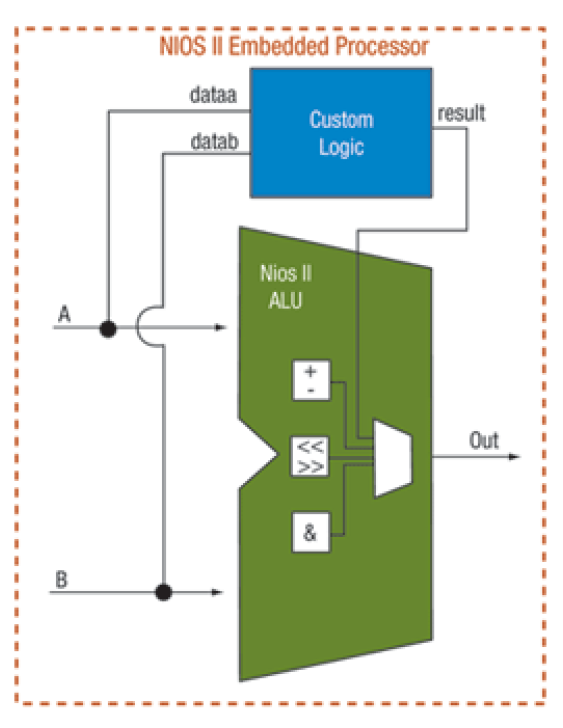
\includegraphics[width=0.9\textwidth]{./pictures/custom_instruction.png} 
		\end{minipage}
		
	\subsection{Types of Custom Instructions}
	
		\begin{compactitem}
		  \item Combinatorial
		  \item Multi-Cycle, synchronised by clock
		  \item Parametrised
		\end{compactitem}
		
		\begin{tabular}{p{0.475\textwidth}p{0.475\textwidth}}
			\vspace{0pt}
			
			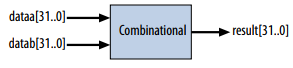
\includegraphics[width=0.8\linewidth]{./pictures/customInstCombinational.png}
			& \vspace{0pt}
			
			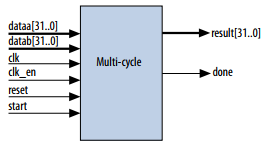
\includegraphics[width=0.8\linewidth]{./pictures/customInstMultiCycle.png}\\
		\end{tabular}
		
	\subsection{Custom instruction Assembly Interface}
		This example shows a call to a custom instruction with the following parameters:
	
		\begin{table}[H]\centering
			\begin{tabular}{ll}
				Selection Index: 
					& 0\\
				Input (\texttt{dataa[31:0]}, \texttt{datab [31:0]}): 
					& Registers \texttt{R7}, \texttt{R8}\\
				Output (\texttt{result[31:0]}): 
					& Register \texttt{R8}\\
			\end{tabular}
		\end{table}
		
		\lstinputlisting[style=ASM]{./src/customInst.asm}

	\subsection{Custom instruction C/C++ Interface}
		\lstinputlisting[style=C]{./src/customInst.c}